\documentclass[journal,onecolumn,]{IEEEtran}

% Packages
\usepackage{times}
\usepackage[pdftex]{graphicx}
\usepackage{amsmath,amssymb,amsopn,amstext,amsfonts}
\usepackage{cancel}
\usepackage[space]{cite}
\usepackage{pdfsync}
\usepackage{balance}
\usepackage{color}
\usepackage{mathtools}
\usepackage{algpseudocode}
\usepackage{algorithm} %\usepackage[ruled,vlined,linesnumbered]{algorithm2e}
\usepackage{bm}
\newtheorem{theorem}{Theorem}
\usepackage{diagbox}
\usepackage{float}
\usepackage{epstopdf}
\usepackage{pifont}
\usepackage{amsmath}
\usepackage{multirow}
\usepackage{url}
\usepackage{verbatim}
\usepackage[linkcolor=black,citecolor=black,urlcolor=black,colorlinks=true]{hyperref}
%\usepackage{enumitem}
\usepackage{booktabs}
\usepackage{graphicx}
\usepackage{subcaption}
\usepackage{threeparttable}  
\usepackage{orcidlink}

\usepackage{algorithm}

\ifCLASSINFOpdf

\title{AWP Token: Bridging CS2 Culture \\ with the Crypto World}
\author{AWP Comunication \\ https://awp-gg.xyz/}
\date{}



\usepackage{titlesec}
\titleformat{\section}[block]{\normalfont\Large\bfseries\filright}{\thesection}{1em}{}
\titleformat{\subsection}[block]{\normalfont\large\bfseries\filright}{\thesubsection}{1em}{}
\titleformat{\subsubsection}[block]{\normalfont\normalsize\bfseries\filright}{\thesubsubsection}{1em}{}

\begin{document}
	
	\maketitle
	
	
	
	\section*{Abstract}
	As cryptocurrencies become increasingly important in societal transactions and structures, the Arctic Warfare Police (AWP) Token has emerged to encapsulate the nostalgic vibes of Counter-Strike 2 (CS2) LAN parties and the high-stakes culture associated with the iconic AWP sniper rifle. The AWP Token is not merely a cryptocurrency; it is a homage to the adrenaline-fueled moments and the risk-reward dynamics that define the AWP and CS2 communities.
	
	\section{Introduction}
	The AWP is a legendary sniper rifle in CS2, revered for its ability to deliver high-risk, high-reward gameplay with its one-shot kill potential. It is more than just a weapon; it is a symbol of mastery and prestige within the gaming community, embodying the nostalgic and thrilling moments of past CS/LAN parties\cite{CSGOBombCode}\cite{PixelsUnderstandingSignificance}.
	
	The AWP Token is crafted to merge the passion for this high-stakes culture with the world of cryptocurrencies\cite{nakamotoBitcoinPeertoPeerElectronic}, creating a bridge between the exhilarating world of esports and the innovative realm of digital currencies. As a blockchain-based meme coin, it serves as a cultural token that celebrates the AWP culture and the intense, nostalgic experiences of the CS2 community.
	
	Moreover, the launch of the AWP Token is about reinforcing a shared identity and sense of belonging among CS2 enthusiasts worldwide. It emphasizes the cultural and communal connections over financial transactions, deepening social interaction both within and outside the game.
	
	By integrating with the world of cryptocurrencies, the AWP Token introduces an innovative mode of community participation. It captures the nostalgia and excitement of CS2 and transforms it into a new social and cultural experience, encouraging players to share their high-stakes gaming experiences and strengthening the bonds within the gaming community.
	
	As the AWP Token evolves, it aims to encapsulate the essence of CS2's competitive spirit and the nostalgic, high-risk, high-reward culture in each cultural exchange. It serves as a recognition of the dedication of those who spend hours honing their skills and the strategists who deftly navigate the high stakes of the game. The AWP Token symbolizes an evolution in gaming culture and an intriguing blend with the culture of cryptocurrencies.
	
	\section{Logo and Base Chain}
	The logo of the AWP Token features the classic AWP sniper rifle from CS2, symbolizing respect and nostalgia for this iconic weapon, as shown in Fig.\ref{pic:1}. The Base chain is chosen to launch the AWP Token, aiming to utilize its efficiency and accessibility while expressing respect for the Ethereum chain as the birthplace of cryptocurrencies.
	
	
	
	\begin{figure*}[b]
		\centering
		\begin{subfigure}{0.45\linewidth}
			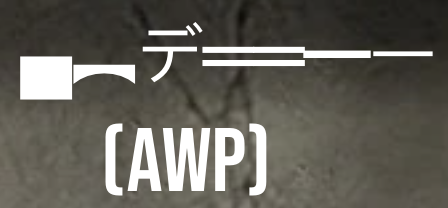
\includegraphics[width=1\linewidth]{figure/1.png}
			\captionsetup{font={small}}
			\caption{AWP Token logo}
			\label{pic:12}
		\end{subfigure}
		\begin{subfigure}{0.45\linewidth}
			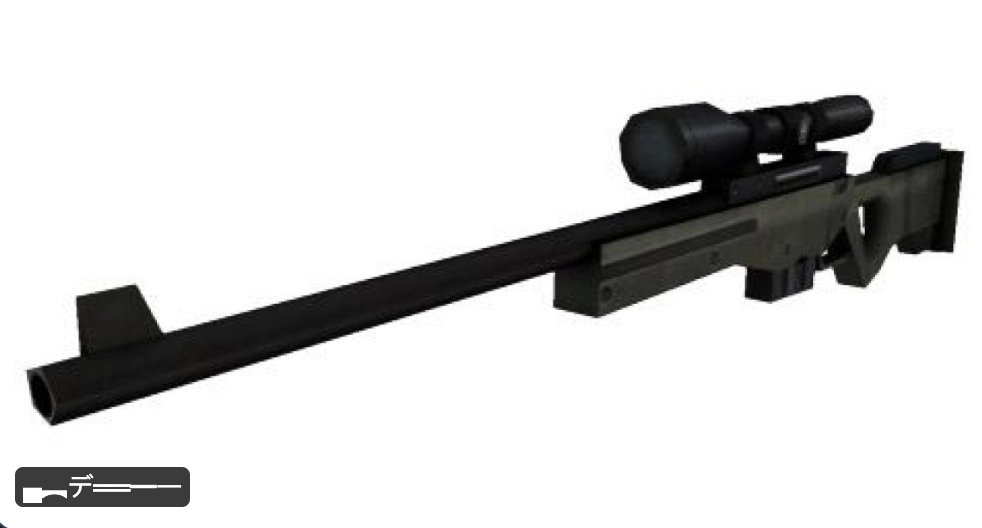
\includegraphics[width=1\linewidth]{figure/3.png}
			\captionsetup{font={small}}
			\caption{Physical representation of the AWP in CS2}
			\label{pic:11}
		\end{subfigure}
		\captionsetup{font={small}}
		\caption{
			AWP Cultural Mapping. a) The logo for the AWP Token, featuring design elements that incorporate the silhouette of the AWP sniper rifle, reflective of the token's connection to the gaming community. b) A detailed depiction of the AWP sniper rifle from CS2, highlighting its distinctive scope, barrel, and stock, symbolic of its power and precision within the game. }
		\label{pic:1}
		\vspace{-0.5cm}
	\end{figure*}
	
	
	

	
	\section{AWP Token Economics}
	
	The total supply of AWP Tokens is set at \textbf{1,000,022} to commemorate the unique status of the AWP in CS2. This supply is fixed and will not increase, ensuring its scarcity and value. The initial liquidity is provided by the project's founders to ensure market liquidity.
	
	AWP Token contract address:
	\begin{center}
		\textbf{0x5e9fE073Df7Ce50E91EB9CBb010B99EF6035a97D}
	\end{center}
	
	The tokens held by the team are protected by a multi-signature wallet on the Base chain with an execution threshold of \textbf{3/4}.
	
	Multi-signature wallet address:
	\begin{center}
		\textbf{0xDf8818C289e863b614Ed04938ba41220c7fA74F8}
	\end{center}
	
	The concentration of token ownership ensures that a focused group of holders, committed to the culture and future of the AWP token, have significant influence on its development. However, it poses potential risks to decentralization. The current distribution of token holders is shown in Fig.\ref{pic:token_distribution}, where \textbf{0x00**dead} represents the burn address, \textbf{0x3c**9577} is the initial liquidity provider address, and \textbf{0xdf**74f8} is the team's multi-signature wallet address.
	
	To demonstrate a long-term commitment, the project initially destroyed the provided liquidity certificates with the following transaction hash:
	\begin{center}
		\textbf{0x6ad33cea6a9a8743eebd87e73aa3fd33b1a6454977c51ac428fef747945215bc}
	\end{center}
	
	Subsequently, to reduce the circulating supply and enhance community trust, multiple supply destruction operations were carried out, totaling \textbf{16.68\%} of the supply. The transaction hashes for these operations are:
	\begin{center}
		\textbf{0xfc487c0d7996e64fde72c9ae16defddc7c17b08ce599da7d975de7ecc1012f36}
		\textbf{0x4bf1c3f7c347c6a52aed57dc17340549febf1edc882988c11c2c0ca3ed19bae3}
		\textbf{0x015f3b7f2e65d1f40d45d00c0c9f91d3ce5ca8e776f2dc09347631366efde60d}
	\end{center}
	
	Additionally, \textbf{5\%} of the AWP supply will be allocated for community and marketing incentives. Community ownership is key, and this is a vital step towards full community takeover.
	
	As the community grows and more tokens are distributed, we hope to see a gradual move towards decentralization, fostering stronger and more diverse community engagement.
	
	\begin{figure}[h]
		\centering
		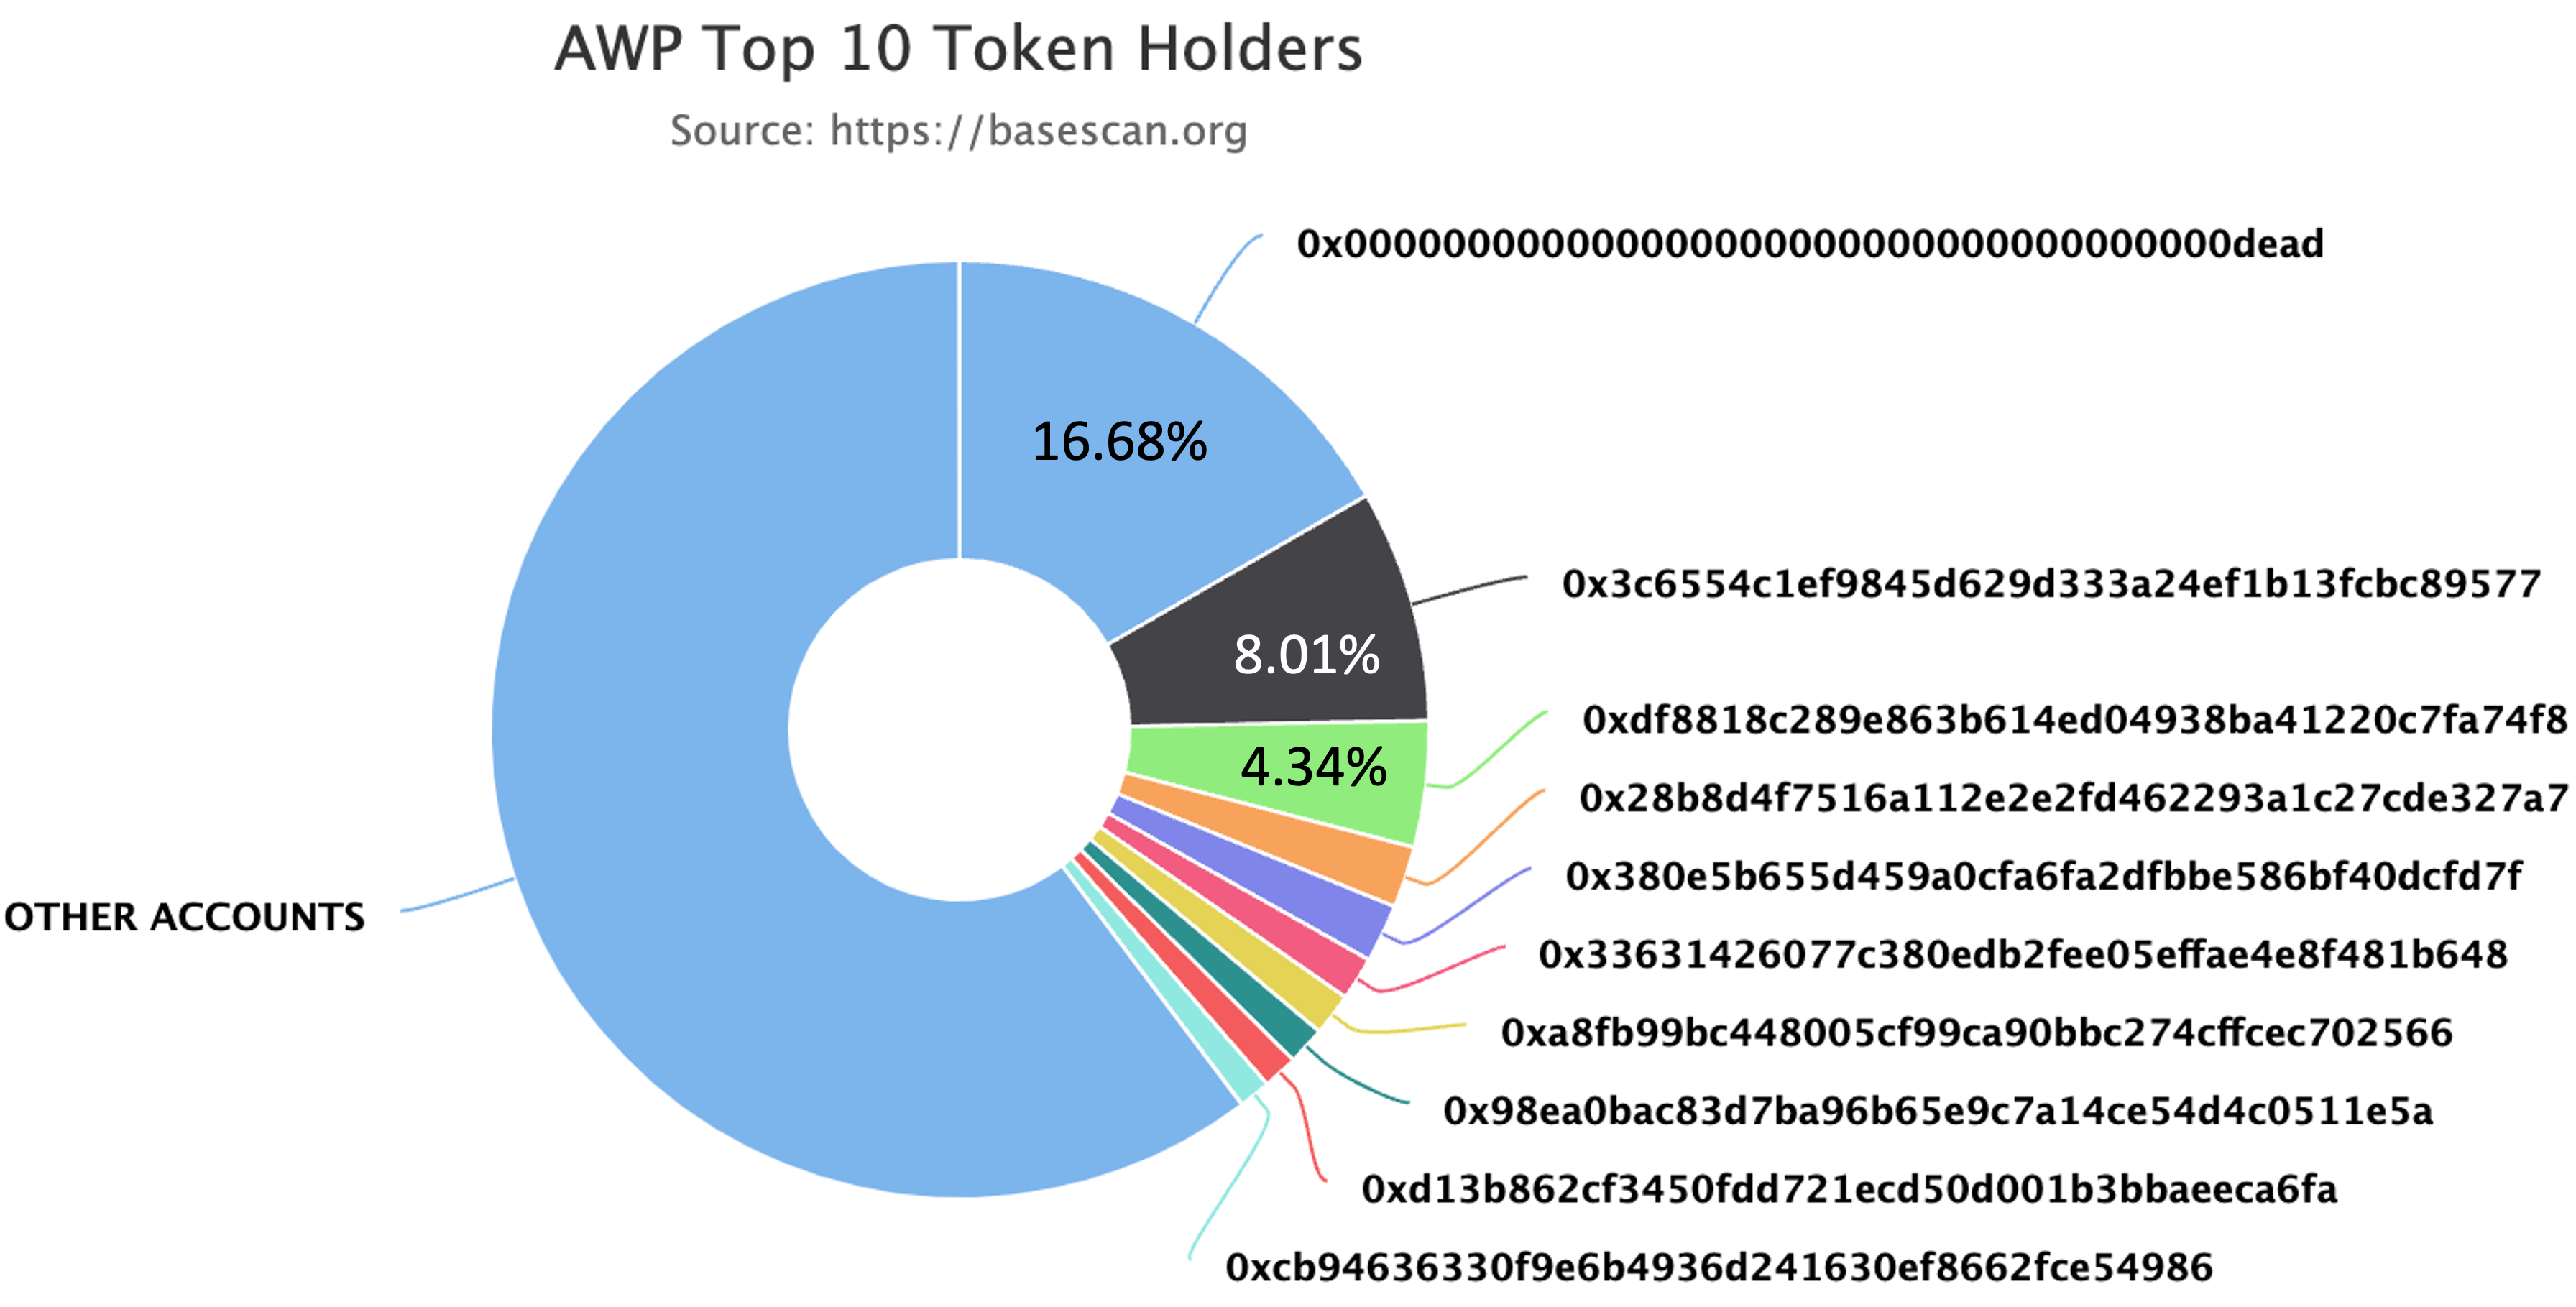
\includegraphics[width=1\linewidth]{figure/token_distribution2.png}
		\caption{Distribution of AWP Tokens among the top 500 holders. The pie chart depicts the share of tokens held by the top accounts relative to the total token supply, highlighting the concentration of ownership. Data source: BaseScan TokenHolderChart, snapshot taken on Monday, April 8, 2024, at 17:43:26 UTC.}
		\label{pic:token_distribution}
	\end{figure}
	

	
	
	\section{Conclusion}
	The launch of the AWP Token is a tribute to the AWP sniper rifle culture in CS2. It is not only a cryptocurrency but also a cultural symbol. It provides a platform for CS2 players and cryptocurrency enthusiasts to communicate and resonate, promoting the spread and development of AWP culture in the crypto world.
	
	
	
	\section*{Disclaimer}
	
	AWP Token is a tribute to the AWP sniper rifle culture in CS2, and it is not designed for profit. The information provided in this article does not constitute financial advice. If you are interested in AWP Token, feel free to participate; if not, that is perfectly fine. If you do not believe or understand, we kindly ask for your understanding, as we may not be able to invest time in detailed explanations.
	
	
	\vfill
	
	\bibliographystyle{IEEEtran} 
	\bibliography{awp2024}
	
	
	
	
\end{document}
